\vspace{12pt}
\section{Structural Characterization of Thin Films}
\subsection{General Crystallographic Characteristics of Doped Thin Films}
X-ray diffraction analysis was used for structural characterization of the thin films grown by PLD in this research. Figure \ref{fig:xrd:films:dopants:oneAxis} shows a series of XRD patterns that highlight the general microstructural features of films grown at a temperature of 850\textdegree C with a laser energy density of 2.8 J/cm$^2$. 
\begin{figure}
    \centering
    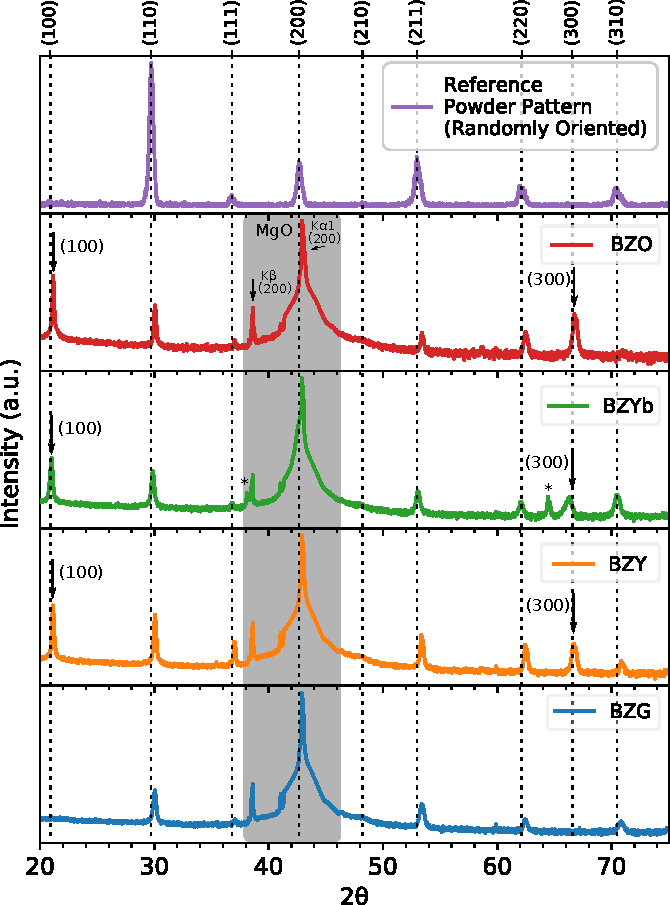
\includegraphics{Figures/190524-xrd-bzo-bzg-bzy-bzyb-thin-films-3-edit.pdf}
    \caption{$\theta$-2$\theta$ scans of thin films deposited on (100)-oriented MgO substrates at a temperature of 850\textdegree C with a laser energy density of 2.8 J/cm$^2$. Ablation targets were prepared by solid state reaction with addition of the various dopants shown. ``BZO'' refers to an undoped BaZrO$_3$ thin film. The reference powder pattern corresponds to a 2$\theta$ scan from a sintered pellet of Gd-doped BaZrO$_3$ and it exhibits the relative intensities typical of a randomly oriented polycrystalline material. Miller indices shown on the top axis of the figure indicate the positions of all reflections of cubic BaZrO$_3$. The shaded area covering the 2$\theta \approx 38$-$45$\textdegree\ range is dominated by the (200) reflection of the single crystal MgO substrate (for both, K$\alpha$ and K$\beta$ lines of the X-ray source). Peaks marked with (*) are from silver contacts applied prior to XRD.}
    \label{fig:xrd:films:dopants:oneAxis}
\end{figure}
The pattern of a bulk BaZrO$_3$ powder sample is included for reference. The reference powder is a polycrystalline bulk sample with randomly oriented grains. Consequently, the shown 2$\theta$ scan exhibits the relative intensities of a randomly oriented polycrystalline material. The $\theta$-2$\theta$ scans of Figure \ref{fig:xrd:films:dopants:oneAxis} show polycrystalline patterns for both, doped and undoped thin films grown at the indicated conditions. This is evident by the presence of virtually all BaZrO$_3$ reflections in the film patterns. The pattern for the undoped film (marked as``BZO'') for example, shows prominent peaks for the (100), (110), (111), (211), (220), and (300) families of planes. Although significantly weaker, the (210) and (310) peaks are also clearly present. The (200) reflection of BaZrO$_3$ is not fully resolved because of its near overlap with the (200) reflection of the MgO substrates, which dominates the $\theta$-2$\theta$ scans in the 2$\theta \approx 38$-$45$\textdegree\ range (indicated by a shaded area in Figure \ref{fig:xrd:films:dopants:oneAxis}). The $\theta$-2$\theta$ of Figure \ref{fig:xrd:films:dopants:oneAxis} also show substantial shifts in the peak positions of the films with respect to the bulk pattern, probably indicative of thin film strain effects. Calculations of lattice parameters for these films show in Table \ref{tab:film:dopant:latticeParam} do not indicate any pattern with dopant ionic radius. 
\begin{table}[b]
    \centering
    \caption{Lattice parameters calculated from the patterns in Figure \ref{fig:xrd:films:dopants:oneAxis} which films deposited on MgO substrates at 850\textdegree C with a laser energy density of 2.8 J/cm$^2$. }
    \begin{tabular}{lr}
        \toprule
        Dopant &  Lattice Parameter \\
        \midrule
        \midrule
          pure &              4.203 \\
            Yb &              4.227 \\
             Y &              4.204 \\
            Gd &              4.205 \\
        \bottomrule
    \end{tabular}
    \label{tab:film:dopant:latticeParam}
\end{table}

One of the most interesting effects revealed by Figure \ref{fig:xrd:films:dopants:oneAxis} is the presence or preferred crystallite orientation in some of the films. The Gd-doped film exhibits relative peak intensities very similar to the bulk powder, indicating an essentially random distribution of grain orientations. On the other hand, the Y- and Yb-doped films (as well as the undoped sample) show the strong emergence of the (100) and (300) reflections. These peaks have very low intensity in a randomly oriented sample. Their dominant presence in the BZO, BZY, and BZYb thin films suggest strong crystallographic texturing effects with crystallites having the [100]-axis of their cubic BaZrO$_3$ structured preferentially aligned with the normal of the substrate. 

\subsection{Effect of Laser Energy Density}
The neutral and ionized species arriving at the crystallization front of a thin film crystal growing during PLD can have kinetic energies in excess of 100 eV. This corresponds to arrival velocity of tens of thousands of centimeters per second. These highly energetic species can have significant impact in the film microstructure, causing crystal configurations that deviate from what would be expected in conditions near thermodynamic equilibrium. An effective PLD parameter in controlling the kinetic energy of these species is the laser energy density. High laser energy densities has been correlated with a variety of thin film effects, including enhanced surface diffusion \cite{Willmott2004}, the generation of stress in thin films \cite{Voevodin1996}, and the promotion of preferred crystallographic orientations \cite{Kim2007}. High laser energy densities also lead to high supersaturations in the plume vapor, which impacts the nucleation rate of new crystallites. Control of supersaturation during PLD is known to cause major shifts in crystal growth mode, permitting access to layer-by-layer atomic growth (Frank-van der Merwe mode typically leading to single crystal films) \cite{Ohtomo2005}, three-dimensional Volmer-Weber island growth mode, which normally leads to polycrystalline material \cite{Rao2014}, and also Stranski-Krastanov growth modes in the case of heteroepitaxy \cite{Norton2004,Weidenkaff2006}.

\begin{figure}
    \centering
    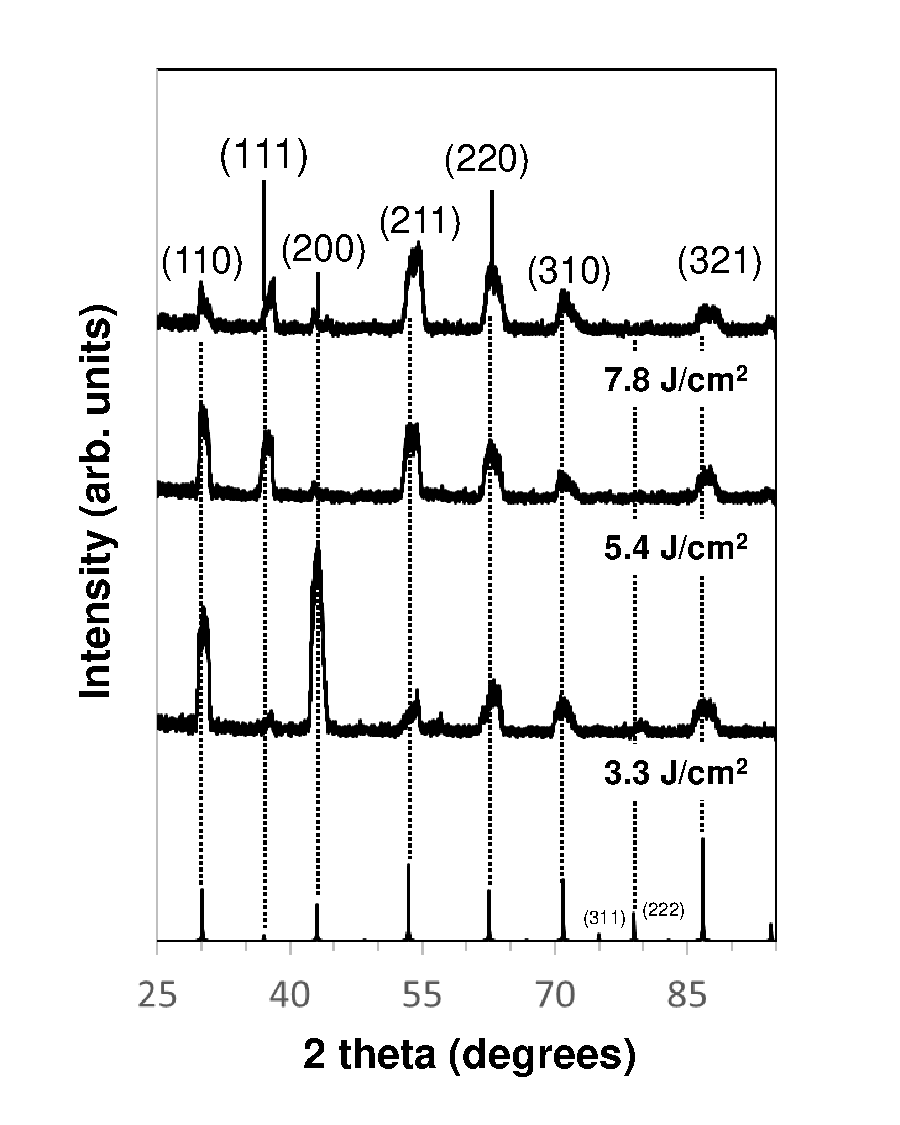
\includegraphics[width=0.7\textwidth]{Figures/Energy_Density_Effect.pdf}
    \caption{2$\theta$ scans of undoped BaZrO$_3$ thin films deposited at 650\textdegree C on silicon substrates using different values of laser energy density.}
    \label{fig:energy_density:effect}
\end{figure}
\begin{figure}
    \centering
    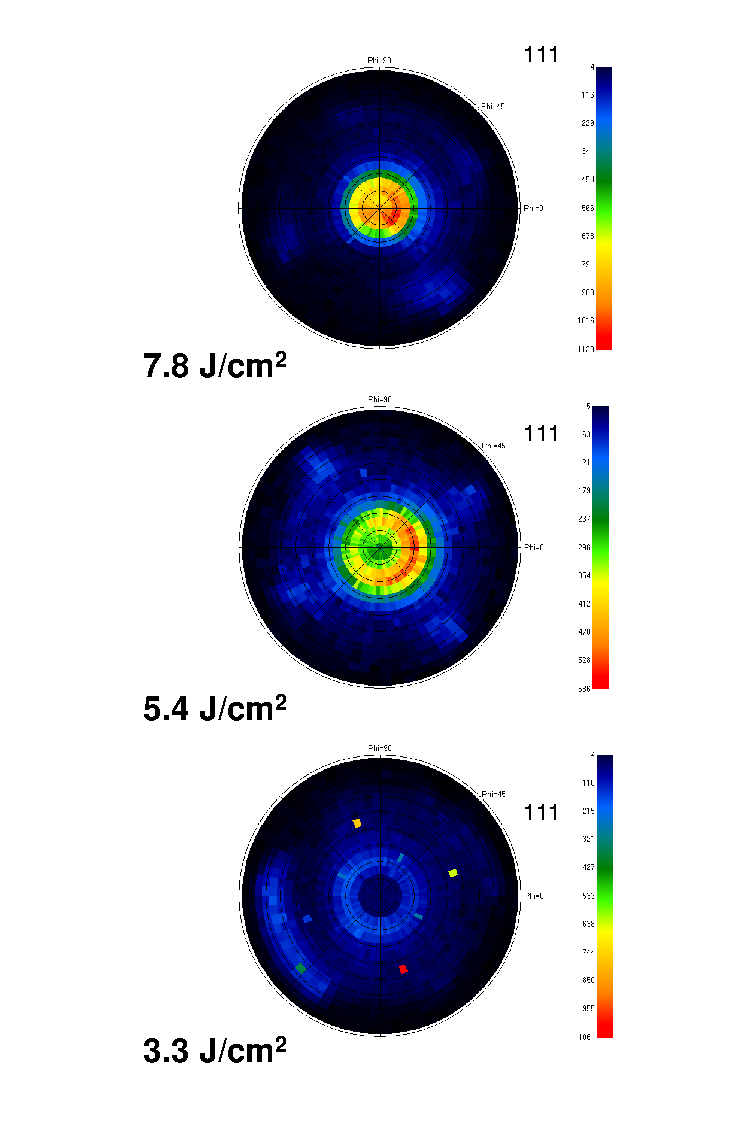
\includegraphics[width=0.6\textwidth]{Figures/Energy_Density_Effect_Pole_Figures.pdf}
    \caption{(111) Pole figures from undoped thin films deposited at 650\textdegree C on silicon substrates using different values of laser energy density.}
    \label{fig:energy_density:effect:pole_figures}
\end{figure}

Thin films have been grown in this research to evaluate the effect of the laser energy density in the film microstructure. Figure \ref{fig:energy_density:effect} shows an example of the effect of energy density in undoped BaZrO$_3$ deposited by PLD on silicon (Si) substrates at a temperature of 650\textdegree C. The relative intensities of the 2$\theta$ patterns deviate significantly from a random polycrystalline pattern. This is particularly evident in the (111) planes of the perovskite structure for the higher laser energy densities of 5.4 J/cm$^2$ and 7.8 J/cm$^2$. These high (111) intensities suggest some texturing effect in this direction. In order to further evaluate this effect, measurements of crystallographic texture were performed on select thin film samples by XRD in reflection geometry using the 3-axes cradle of a Panalytical Empyrean diffractometer. X-ray pole figures were collected for select reflections of BaZrO$_3$ by varying the polar angle ranging from 0\textdegree\ to 85\textdegree\ and the azimuthal angle ranging from 0\textdegree\ to 360\textdegree\ with a step increment of 5\textdegree\ and a scan time of 4 s per step. The pole figures were not corrected for background and defocusing of the incident beam, and therefore represent a qualitative assessment of general texturing trend in the analyzed thin films. Figure \ref{fig:energy_density:effect:pole_figures} shows pole figures obtained for the [111] poles for the same samples of Figure \ref{fig:energy_density:effect}. 
The density of crystallites with [111] poles oriented along the direction normal to the substrate clearly increases with the laser energy density. The amorphous layer of native oxide on the Si substrates rules out the substrate as a driving force for epitaxy in these samples. These results indicate the potential of the PLD technique to grow BaZrO$_3$ thin films with crystallographic texture in unusual orientations that could be useful for harnessing ionic conductivity properties.  

\vspace{12pt}
\subsection{Effect of Deposition Temperature}
\label{sec:film:xrd:epitaxy}
The deposition temperature is one of the most significant parameters in thin film crystal growth during PLD. In order to investigate its impact on the growth of doped BaZrO$_3$, thin films were deposited while applying different temperatures on our radiatively-heated substrate holder. In this study, (100)-oriented single crystalline magnesium oxide (MgO) was chosen as a substrate material. This substrate was chosen for its excellent match of lattice parameter (4.212 \AA) to barium zirconate (4.196 \AA). This nearly ideal lattice matching could provide a way to grow the material in large grains without stress from the substrate as well as the possibility of epitaxial rather than polycrystalline growth from the substrate. In addition, due to its excellent electric and ionic insulating properties, it provides a way to test the conductivity of the thin films grown on it without any contribution from its own conductive processes.

Concentrating on the Gd-doped thin films, Figure \ref{fig:film:xrd:2theta} shows 2$\theta$ scans of films grown at different temperatures using a laser energy density of 2.8 J/cm$^2$. The thin film grown at 750\textdegree C exhibits a pattern that is not too different from a random polycrystalline material (although the relative intensities of the (110) and (200) reflections are somewhat altered). A significant change is observed however for the growth temperatures of 850\textdegree C and 950\textdegree C. For the same laser energy densities and XRD data acquisition conditions, one observes the greatly diminished polycrystalline reflections in the 850\textdegree C sample, and total absence of peaks in the 950\textdegree C film. The essentially unchanged background indicates that the absence of crystalline peaks in the higher temperature sample is unlikely to be due to film amorphization. An alternative explanation would be the growth of single crystals or highly-texture films, for which the Bragg diffraction condition is no longer met in the 2$\theta$ scan. Figure \ref{fig:film:xrd:2theta:log} shows a re-plot of the data in Figure \ref{fig:film:xrd:2theta} in a log scale on the vertical axis, which emphasizes the substantial reduction (more than one order of magnitude) in the peak intensities of the 850\textdegree C sample with respect to the 750\textdegree C film, and the absence of reflections at 950\textdegree C.

\begin{figure}

    \centering
    \begin{subfigure}[b]{0.45\linewidth}
        
        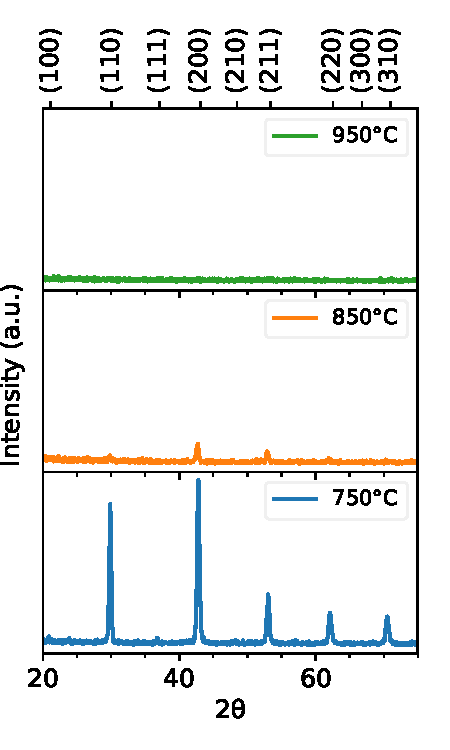
\includegraphics[width=\linewidth]{Figures/180316-thin-film-2theta.pdf}
        \caption{}
        \label{fig:film:xrd:2theta}
    \end{subfigure}\hspace{.125in}
    \begin{subfigure}[b]{0.45\linewidth}
        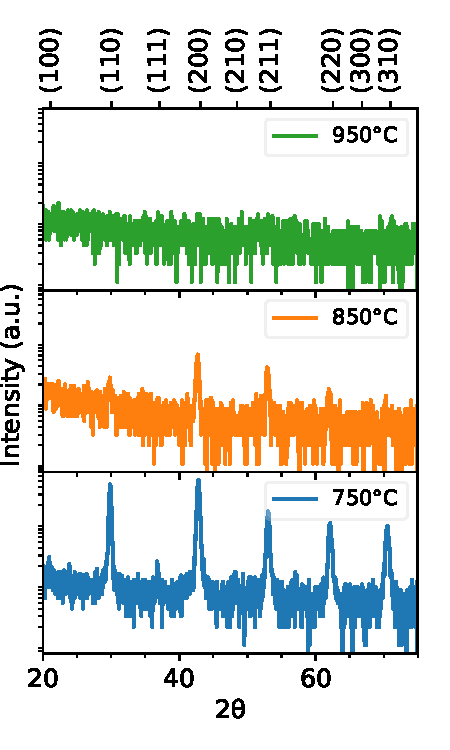
\includegraphics[width=\linewidth]{Figures/180316-thin-film-2theta-log.pdf}
        \caption{}
        \label{fig:film:xrd:2theta:log}
    \end{subfigure}
    \caption{(A) 2$\theta$ scans of thin films deposited on (100)-oriented MgO substrates at the indicated temperatures. Films grown during ablation of a Gd-doped target prepared by chemical spray pyrolysis using a laser energy density of 2.8 J/cm$^2$. Miller indices shown on the top axis of the figure indicate the positions of all reflections of cubic BaZrO$_3$. (B) is plotted on the log scale.}
\end{figure}

\begin{figure}
    \centering
    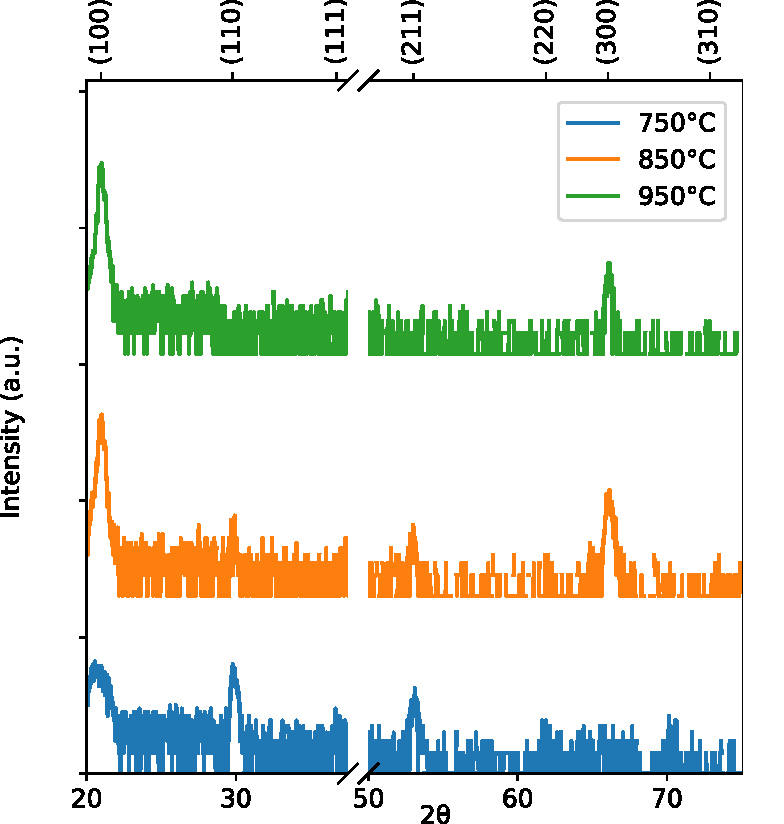
\includegraphics{Figures/180316-thin-film-2thetaOmega-sym-logplot-broken-axes-indexed-edit-2.pdf}
    \caption{$\theta$-2$\theta$ scans of thin films deposited on (100)-oriented MgO substrates at the indicated temperatures. Films grown during ablation of a Gd-doped target prepared by chemical spray pyrolysis using a laser energy density of 2.8 J/cm$^2$. Miller indices shown on the top axis of the figure indicate the positions of all reflections of cubic BaZrO$_3$. A break was introduced in the horizontal in the 2$\theta= 40$-$50$\textdegree\ range to remove the large (200) reflection of the single crystal MgO substrate.}
    \label{fig:films:xrd:2thetaOmega:brokenAxis}
\end{figure}

\begin{figure}
 \centering
    \begin{subfigure}[t]{.45\linewidth}
        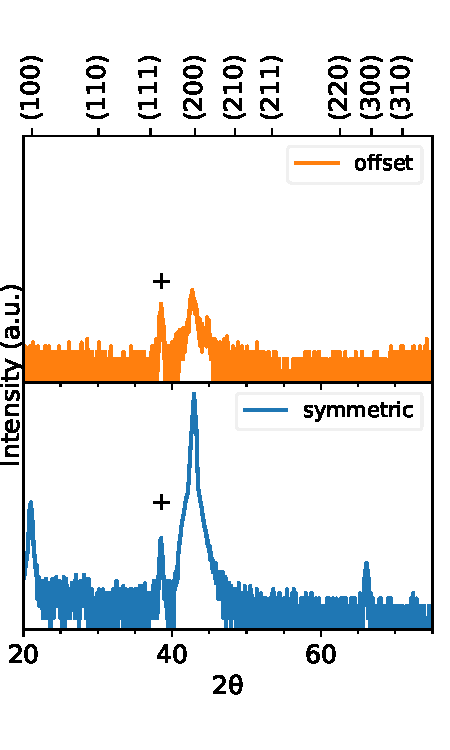
\includegraphics[width=\linewidth]{Figures/180316-film-950-2thetaOmegaOffset.pdf}
        \caption{}
        \label{fig:films:xrd:2thetaOmega:offset:950}
    \end{subfigure}\hspace{.125in}
    \begin{subfigure}[t]{.45\linewidth}
        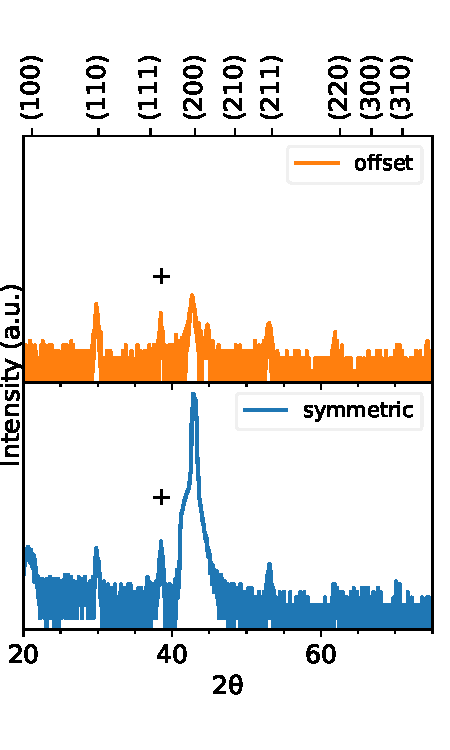
\includegraphics[width=\linewidth]{Figures/180316-film-750-2thetaOmegaOffset.pdf}
        \caption{}
        \label{fig:films:xrd:2thetaOmega:offset:750}
    \end{subfigure}
    \caption{(A) $\theta$-2$\theta$ (symmetric) scan of the 950\textdegree C Gd-doped film and corresponding asymmetric $\omega$-2$\theta$ scan with an offset $\phi =  2$\textdegree. The peaks from lattice planes parallel to the c-axis are diminished or absent due to the offset. (B) $\theta$-2$\theta$ (symmetric) scan of the 750\textdegree C Gd-doped film and corresponding asymmetric $\omega$-2$\theta$ scan with an offset $\phi =  2$\textdegree. Peaks from polycrystalline grains are unaffected by the offset in scanning angle. The prominent substrate peak at 42\textdegree\ also diminishes under asymmetric scanning due to its single crystalline nature.  Another substrate peak (caused by diffraction of the K$\beta$ line of the X-ray source by the (200) planes) is marked by a cross (+).}
    \label{fig:films:xrd:2thetaOmega:offset}
\end{figure}
The growth of a single crystal, or highly textured epitaxially-oriented thin film at 950\textdegree C, is confirmed by the $\theta$-2$\theta$ scan shown in Figure \ref{fig:films:xrd:2thetaOmega:brokenAxis}. For the samples grown at 750\textdegree C and 850\textdegree C, the $\theta$-2$\theta$ patterns yield clear peaks for many of the BaZrO$_3$ reflections, indicating grains in many different orientations. The different peak intensities seen when comparing the 750\textdegree C and the 850\textdegree C samples suggest different degrees of crystallographic texture. In the case of the film grown at 950\textdegree C, however, it is clear that only the peaks of the (100) and (300) families of planes are present. A (200) reflection for the film is also present but difficult to resolve due to overlap with the large (200) peak of MgO substrate, which is removed from the plot of Figure \ref{fig:films:xrd:2thetaOmega:brokenAxis}.

Further confirmation of the epitaxial orientation of the 950\textdegree C film is provided by the data in Figure \ref{fig:films:xrd:2thetaOmega:offset:950}. A comparison between the  $\theta$-2$\theta$ (symmetric) scan and an asymmetric $\omega$-2$\theta$ shows the complete disappearance of the (100) and (300) reflections of the oriented phase when a small offset of $\phi = 2$\textdegree\ is added to the incident angle $\omega$. The only peak remaining in the asymmetric scan is the (200) reflection from the substrate. A shoulder riding on the low-angle side of the substrate peak also vanishes in the asymmetric scan.  

Overall, Figures \ref{fig:film:xrd:2theta} through \ref{fig:films:xrd:2thetaOmega:offset:750} indicate that at low deposition temperatures, polycrystalline microstructure develops, but that at high deposition temperature,  highly textured growth occurs leading to epitaxially oriented thin films on lattice matched single crystal MgO substrate.